Substituting
\begin{align}
	 r = \sqrt{2},\
	\vec{u}
	 = \myvec{-1\\-1}
\end{align}
in 
	\eqref{eq:circ-cr},
\begin{align}
	f 
	  =0	
\end{align}
Thus, the equation of the circle is 
\begin{align}
	\norm{\vec{x}}^2 -2\myvec{1&1}\vec{x} = 0       		       
\end{align}	
See 
\figref{fig:chapters/11/11/1/4/Fig1}.
\begin{figure}[H]
	\begin{center} 
	  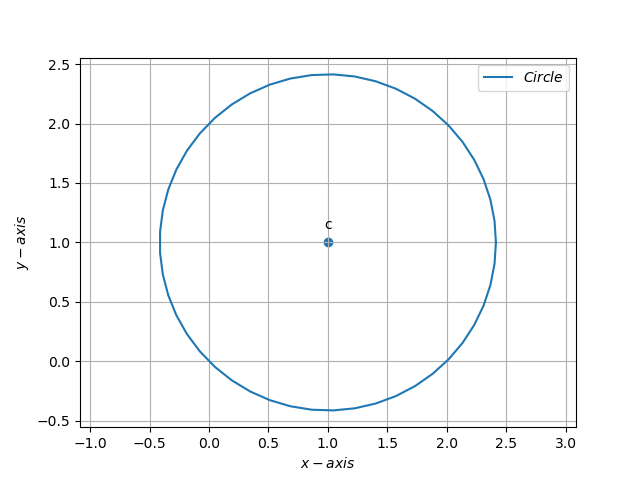
\includegraphics[width=0.75\columnwidth]{chapters/11/11/1/4/figs/circ.png}
	\end{center}
\caption{}
\label{fig:chapters/11/11/1/4/Fig1}
\end{figure}
